\documentclass{standalone}
\usepackage{tikz}
\usetikzlibrary{patterns}
\usetikzlibrary{positioning}
\usetikzlibrary{patterns, positioning}
\usetikzlibrary{shapes.misc}
\usepackage[outline]{contour}
\contourlength{1.5pt} 
\usepackage[sfdefault]{ClearSans}

\begin{document}
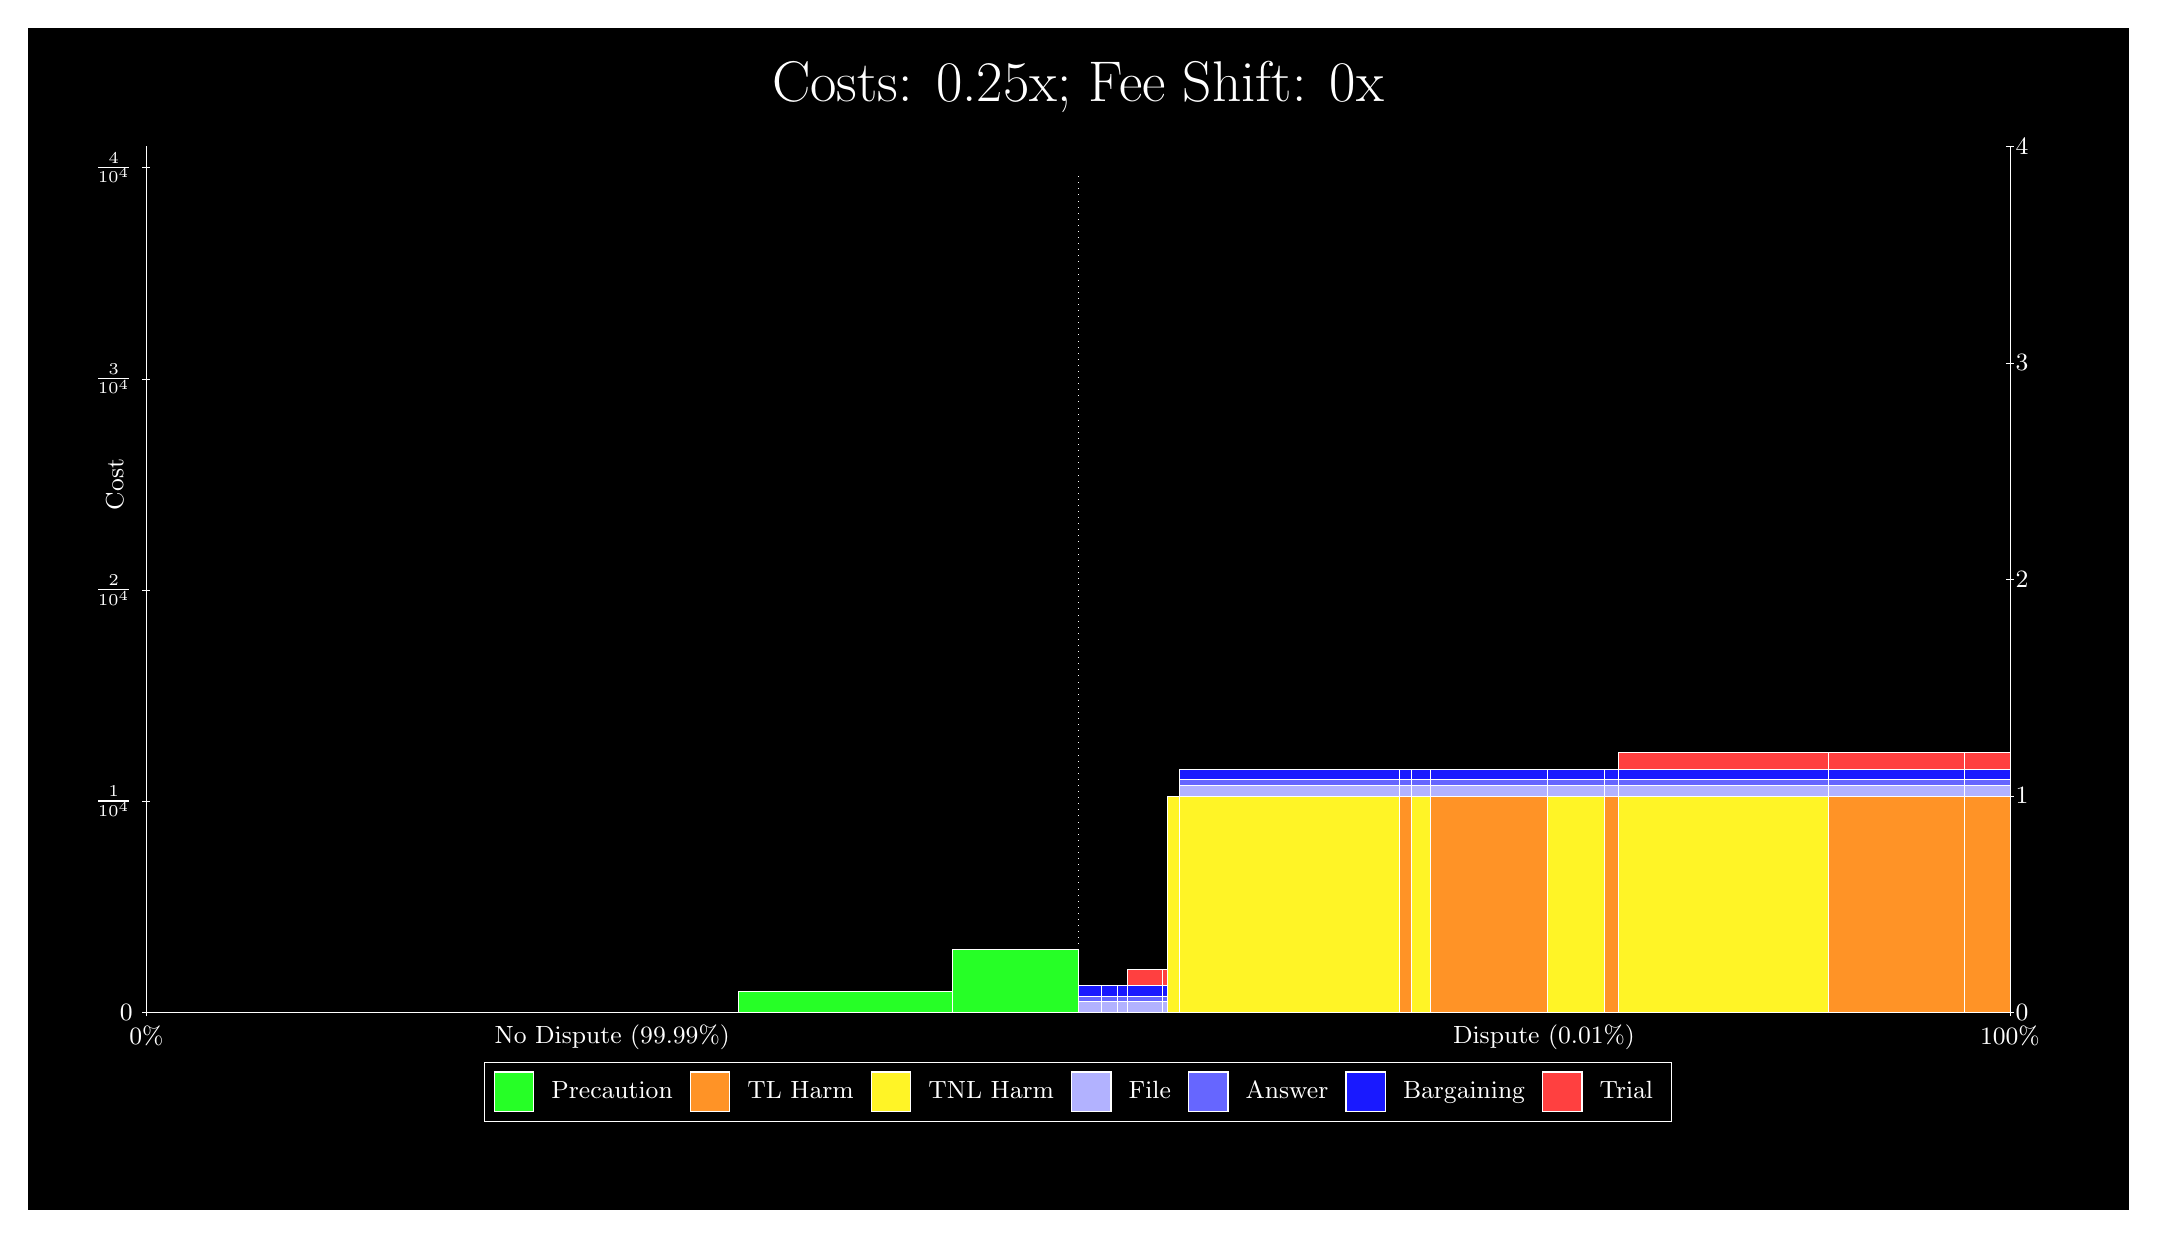
\begin{tikzpicture}
\draw[fill=black] (0,0) rectangle (26.667,15);
\draw[draw=none,text=white] (0,13.5) rectangle (26.667,15) node[midway] {\huge Costs: 0.25x; Fee Shift: 0x };
\draw[fill=green!85,draw=white,very thin] (9.0126,2.5) rectangle (11.735,2.7682);
\draw[fill=green!85,draw=white,very thin] (11.735,2.5) rectangle (13.333,3.3047);
\draw[fill=blue!30,draw=white,very thin] (13.333,2.5) rectangle (13.628,2.6375);
\draw[fill=blue!60,draw=white,very thin] (13.333,2.6375) rectangle (13.628,2.7063);
\draw[fill=blue!90,draw=white,very thin] (13.333,2.7063) rectangle (13.628,2.8438);
\draw[fill=green!85,draw=white,very thin] (13.628,2.5) rectangle (13.826,2.5);
\draw[fill=blue!30,draw=white,very thin] (13.628,2.5) rectangle (13.826,2.6375);
\draw[fill=blue!60,draw=white,very thin] (13.628,2.6375) rectangle (13.826,2.7063);
\draw[fill=blue!90,draw=white,very thin] (13.628,2.7063) rectangle (13.826,2.8438);
\draw[fill=green!85,draw=white,very thin] (13.826,2.5) rectangle (13.961,2.5001);
\draw[fill=blue!30,draw=white,very thin] (13.826,2.5001) rectangle (13.961,2.6376);
\draw[fill=blue!60,draw=white,very thin] (13.826,2.6376) rectangle (13.961,2.7063);
\draw[fill=blue!90,draw=white,very thin] (13.826,2.7063) rectangle (13.961,2.8438);
\draw[fill=blue!30,draw=white,very thin] (13.961,2.5) rectangle (14.4,2.6375);
\draw[fill=blue!60,draw=white,very thin] (13.961,2.6375) rectangle (14.4,2.7063);
\draw[fill=blue!90,draw=white,very thin] (13.961,2.7063) rectangle (14.4,2.8438);
\draw[fill=red!75,draw=white,very thin] (13.961,2.8438) rectangle (14.4,3.05);
\draw[fill=green!85,draw=white,very thin] (14.4,2.5) rectangle (14.467,2.5);
\draw[fill=blue!30,draw=white,very thin] (14.4,2.5) rectangle (14.467,2.6375);
\draw[fill=blue!60,draw=white,very thin] (14.4,2.6375) rectangle (14.467,2.7063);
\draw[fill=blue!90,draw=white,very thin] (14.4,2.7063) rectangle (14.467,2.8438);
\draw[fill=red!75,draw=white,very thin] (14.4,2.8438) rectangle (14.467,3.05);
\draw[fill=green!85,draw=white,very thin] (14.467,2.5) rectangle (14.622,2.5001);
\draw[fill=yellow!85,draw=white,very thin] (14.467,2.5001) rectangle (14.622,5.2501);
\draw[fill=yellow!85,draw=white,very thin] (14.622,2.5) rectangle (17.415,5.25);
\draw[fill=blue!30,draw=white,very thin] (14.622,5.25) rectangle (17.415,5.3875);
\draw[fill=blue!60,draw=white,very thin] (14.622,5.3875) rectangle (17.415,5.4563);
\draw[fill=blue!90,draw=white,very thin] (14.622,5.4563) rectangle (17.415,5.5937);
\draw[fill=orange!85,draw=white,very thin] (17.415,2.5) rectangle (17.565,5.25);
\draw[fill=blue!30,draw=white,very thin] (17.415,5.25) rectangle (17.565,5.3875);
\draw[fill=blue!60,draw=white,very thin] (17.415,5.3875) rectangle (17.565,5.4563);
\draw[fill=blue!90,draw=white,very thin] (17.415,5.4563) rectangle (17.565,5.5937);
\draw[fill=green!85,draw=white,very thin] (17.565,2.5) rectangle (17.812,2.5);
\draw[fill=yellow!85,draw=white,very thin] (17.565,2.5) rectangle (17.812,5.25);
\draw[fill=blue!30,draw=white,very thin] (17.565,5.25) rectangle (17.812,5.3875);
\draw[fill=blue!60,draw=white,very thin] (17.565,5.3875) rectangle (17.812,5.4563);
\draw[fill=blue!90,draw=white,very thin] (17.565,5.4563) rectangle (17.812,5.5938);
\draw[fill=green!85,draw=white,very thin] (17.812,2.5) rectangle (19.297,2.5);
\draw[fill=orange!85,draw=white,very thin] (17.812,2.5) rectangle (19.297,5.25);
\draw[fill=blue!30,draw=white,very thin] (17.812,5.25) rectangle (19.297,5.3875);
\draw[fill=blue!60,draw=white,very thin] (17.812,5.3875) rectangle (19.297,5.4563);
\draw[fill=blue!90,draw=white,very thin] (17.812,5.4563) rectangle (19.297,5.5938);
\draw[fill=green!85,draw=white,very thin] (19.297,2.5) rectangle (20.015,2.5001);
\draw[fill=yellow!85,draw=white,very thin] (19.297,2.5001) rectangle (20.015,5.2501);
\draw[fill=blue!30,draw=white,very thin] (19.297,5.2501) rectangle (20.015,5.3876);
\draw[fill=blue!60,draw=white,very thin] (19.297,5.3876) rectangle (20.015,5.4563);
\draw[fill=blue!90,draw=white,very thin] (19.297,5.4563) rectangle (20.015,5.5938);
\draw[fill=green!85,draw=white,very thin] (20.015,2.5) rectangle (20.197,2.5001);
\draw[fill=orange!85,draw=white,very thin] (20.015,2.5001) rectangle (20.197,5.2501);
\draw[fill=blue!30,draw=white,very thin] (20.015,5.2501) rectangle (20.197,5.3876);
\draw[fill=blue!60,draw=white,very thin] (20.015,5.3876) rectangle (20.197,5.4563);
\draw[fill=blue!90,draw=white,very thin] (20.015,5.4563) rectangle (20.197,5.5938);
\draw[fill=yellow!85,draw=white,very thin] (20.197,2.5) rectangle (22.854,5.25);
\draw[fill=blue!30,draw=white,very thin] (20.197,5.25) rectangle (22.854,5.3875);
\draw[fill=blue!60,draw=white,very thin] (20.197,5.3875) rectangle (22.854,5.4563);
\draw[fill=blue!90,draw=white,very thin] (20.197,5.4563) rectangle (22.854,5.5937);
\draw[fill=red!75,draw=white,very thin] (20.197,5.5937) rectangle (22.854,5.8);
\draw[fill=orange!85,draw=white,very thin] (22.854,2.5) rectangle (24.583,5.25);
\draw[fill=blue!30,draw=white,very thin] (22.854,5.25) rectangle (24.583,5.3875);
\draw[fill=blue!60,draw=white,very thin] (22.854,5.3875) rectangle (24.583,5.4563);
\draw[fill=blue!90,draw=white,very thin] (22.854,5.4563) rectangle (24.583,5.5937);
\draw[fill=red!75,draw=white,very thin] (22.854,5.5937) rectangle (24.583,5.8);
\draw[fill=green!85,draw=white,very thin] (24.583,2.5) rectangle (24.588,2.5);
\draw[fill=yellow!85,draw=white,very thin] (24.583,2.5) rectangle (24.588,5.25);
\draw[fill=blue!30,draw=white,very thin] (24.583,5.25) rectangle (24.588,5.3875);
\draw[fill=blue!60,draw=white,very thin] (24.583,5.3875) rectangle (24.588,5.4563);
\draw[fill=blue!90,draw=white,very thin] (24.583,5.4563) rectangle (24.588,5.5938);
\draw[fill=red!75,draw=white,very thin] (24.583,5.5938) rectangle (24.588,5.8);
\draw[fill=green!85,draw=white,very thin] (24.588,2.5) rectangle (25.167,2.5);
\draw[fill=orange!85,draw=white,very thin] (24.588,2.5) rectangle (25.167,5.25);
\draw[fill=blue!30,draw=white,very thin] (24.588,5.25) rectangle (25.167,5.3875);
\draw[fill=blue!60,draw=white,very thin] (24.588,5.3875) rectangle (25.167,5.4563);
\draw[fill=blue!90,draw=white,very thin] (24.588,5.4563) rectangle (25.167,5.5938);
\draw[fill=red!75,draw=white,very thin] (24.588,5.5938) rectangle (25.167,5.8);
\draw[white,very thin] (1.5,2.5) -- (1.5,13.5);
\node[font=\small,rotate=90,text=white, anchor=center] at (1.1, 9.2056) {Cost};
\draw[white,very thin] (1.45,2.5) -- (1.55,2.5);
\node[font=\small,text=white, anchor=east] at (1.45, 2.5) {0};
\draw[white,very thin] (1.45,5.1822) -- (1.55,5.1822);
\node[font=\small,text=white, anchor=east] at (1.45, 5.1822) {$\frac{1}{10^{4}}$};
\draw[white,very thin] (1.45,7.8645) -- (1.55,7.8645);
\node[font=\small,text=white, anchor=east] at (1.45, 7.8645) {$\frac{2}{10^{4}}$};
\draw[white,very thin] (1.45,10.547) -- (1.55,10.547);
\node[font=\small,text=white, anchor=east] at (1.45, 10.547) {$\frac{3}{10^{4}}$};
\draw[white,very thin] (1.45,13.229) -- (1.55,13.229);
\node[font=\small,text=white, anchor=east] at (1.45, 13.229) {$\frac{4}{10^{4}}$};

\draw[white,dotted,very thin] (13.333,2.83) -- (13.333,13.17);
\draw[white,very thin] (25.167,2.5) -- (25.167,13.5);
\draw[white,very thin] (25.117,2.5) -- (25.217,2.5);
\node[font=\small,text=white, anchor=west] at (25.117, 2.5) {0};
\draw[white,very thin] (25.117,5.25) -- (25.217,5.25);
\node[font=\small,text=white, anchor=west] at (25.117, 5.25) {1};
\draw[white,very thin] (25.117,8) -- (25.217,8);
\node[font=\small,text=white, anchor=west] at (25.117, 8) {2};
\draw[white,very thin] (25.117,10.75) -- (25.217,10.75);
\node[font=\small,text=white, anchor=west] at (25.117, 10.75) {3};
\draw[white,very thin] (25.117,13.5) -- (25.217,13.5);
\node[font=\small,text=white, anchor=west] at (25.117, 13.5) {4};

\draw[white,very thin] (1.5,2.5) -- (25.167,2.5);
\draw[white,very thin] (1.5,2.45) -- (1.5,2.55);
\node[font=\small,text=white, anchor=north] at (1.5, 2.45) {0\%};
\draw[white,very thin] (25.167,2.45) -- (25.167,2.55);
\node[font=\small,text=white, anchor=north] at (25.167, 2.45) {100\%};

\node[font=\small,text=white,anchor=south] at (7.4167, 1.9) {No\ Dispute\ (99.99\%)};
\node[font=\small,text=white,anchor=south] at (19.25, 1.9) {Dispute\ (0.01\%)};
\draw (13.3333,2.5) node (B) {};
\begin{scope}[align=center]
\matrix[scale=0.5,draw=white,below=0.5cm of B,nodes={draw},column sep=0.1cm]{
\node[rectangle,draw,minimum width=0.5cm,minimum height=0.5cm,fill=green!85]{}; & \node[draw=none,font=\small,text=white]{Precaution}; &
\node[rectangle,draw,minimum width=0.5cm,minimum height=0.5cm,fill=orange!85]{}; & \node[draw=none,font=\small,text=white]{TL Harm}; &
\node[rectangle,draw,minimum width=0.5cm,minimum height=0.5cm,fill=yellow!85]{}; & \node[draw=none,font=\small,text=white]{TNL Harm}; &
\node[rectangle,draw,minimum width=0.5cm,minimum height=0.5cm,fill=blue!30]{}; & \node[draw=none,font=\small,text=white]{File}; &
\node[rectangle,draw,minimum width=0.5cm,minimum height=0.5cm,fill=blue!60]{}; & \node[draw=none,font=\small,text=white]{Answer}; &
\node[rectangle,draw,minimum width=0.5cm,minimum height=0.5cm,fill=blue!90]{}; & \node[draw=none,font=\small,text=white]{Bargaining}; &
\node[rectangle,draw,minimum width=0.5cm,minimum height=0.5cm,fill=red!75]{}; & \node[draw=none,font=\small,text=white]{Trial}; \\\\
};\end{scope}

\end{tikzpicture}
\end{document}